% =============================================================
%  Angular stability
%  Figures in fig/, copied from presentation/design/ac-transmission/fig/
%  (as_*.pdf), generated by that folder's angular_stability_figures.py
%  from the exact two-port equations.  Worked line: the 500 kV
%  reference line of Section 6.
% =============================================================
\subsection{Angular Stability}
\label{sec:angular-stability}

Section~\ref{sec:limits} introduced the angular criterion as one of three
bounds. On any line long enough to matter it is the one that binds, and the
margin it needs is larger than the criterion alone suggests.

\subsubsection{Synchronising power}
\label{sec:as-ks}

The meaningful quantity is not the crest of the power-angle curve but its
slope, the \emph{synchronising power coefficient}
\begin{equation}
  K_s = \frac{\partial P}{\partial \delta}
      = \frac{U_S \cdot U_R}{X} \cdot \cos\delta
  \label{eq:as-ks}
\end{equation}
which is the stiffness of the electrical coupling between the machines at
either end. Below the maximum, a rotor that advances delivers more power,
decelerates and returns --- negative feedback. Beyond it, advancing delivers
less power and the machine accelerates further; $K_s = 0$ at the maximum is
therefore the steady-state stability limit in the strict sense.
Figure~\ref{fig:as-power-angle} shows both curves for the reference line.

\begin{figure}[!ht]
  \centering
  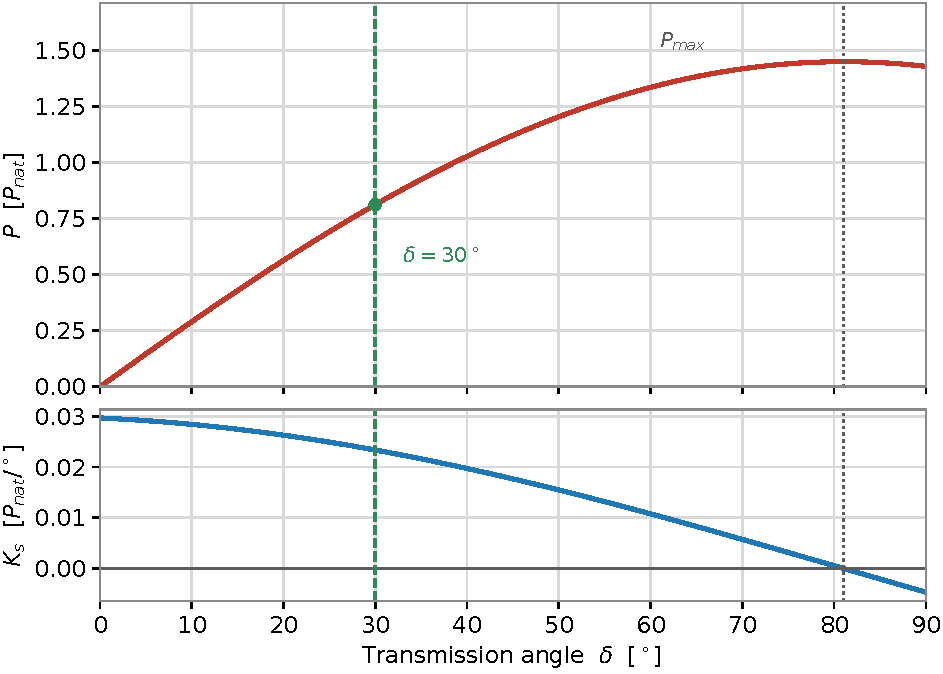
\includegraphics[width=0.74\linewidth]{ac-transmission/fig/as_power_angle.pdf}
  \caption{Power-angle relation and synchronising power coefficient of the
           500\,kV reference line at 300\,mi, both terminals at 1.0\,p.u.}
  \label{fig:as-power-angle}
\end{figure}

With losses the maximum does not fall at $90^\circ$ but at $\delta =
\vartheta_B$, which is $81.0^\circ$ on the reference line. At $\delta =
30^\circ$ the line carries $0.81 \cdot P_{nat}$ with 79\,\% of the stiffness
it has at $\delta = 0$.

Linearising the swing equation about an operating point gives
\begin{equation}
  \frac{2 \cdot H}{\omega_0} \cdot \Delta\ddot{\delta}
  + K_D \cdot \Delta\dot{\delta}
  + K_s \cdot \Delta\delta = 0
  \qquad
  \omega_n = \sqrt{\frac{K_s \cdot \omega_0}{2 \cdot H}}
  \label{eq:as-swing}
\end{equation}
with $H$ the inertia constant and $K_D$ the damping torque coefficient. As
$\delta$ grows, $K_s$ falls, the electromechanical mode slows and its
damping ratio drops. The machine becomes slow and poorly damped before it
loses synchronism, which is why the operating point is held below the
maximum.

\subsubsection{Electrical length}
\label{sec:as-electrical-length}

Above about 250\,km the lumped $\omega \cdot L' \cdot l$
overstates the reactance. The series element of the exact equivalent is
$X' = Z_w \cdot \sin\left(\beta \cdot l\right)$, and substituting into the
lossless maximum gives a clean result:
\begin{equation}
  P_{max} = \frac{U^2}{Z_w \cdot \sin\left(\beta \cdot l\right)}
          = \frac{P_{nat}}{\sin\left(\beta \cdot l\right)}
  \label{eq:as-electrical-length}
\end{equation}
At a quarter wavelength --- 1234\,km on the reference line at 60\,Hz --- the
maximum transfer is exactly $P_{nat}$. That is the analytical spine beneath
the St.~Clair curve, and the reason capability decays with length rather
than staying flat. Figure~\ref{fig:as-electrical-length} compares the three
against length.

\begin{figure}[!ht]
  \centering
  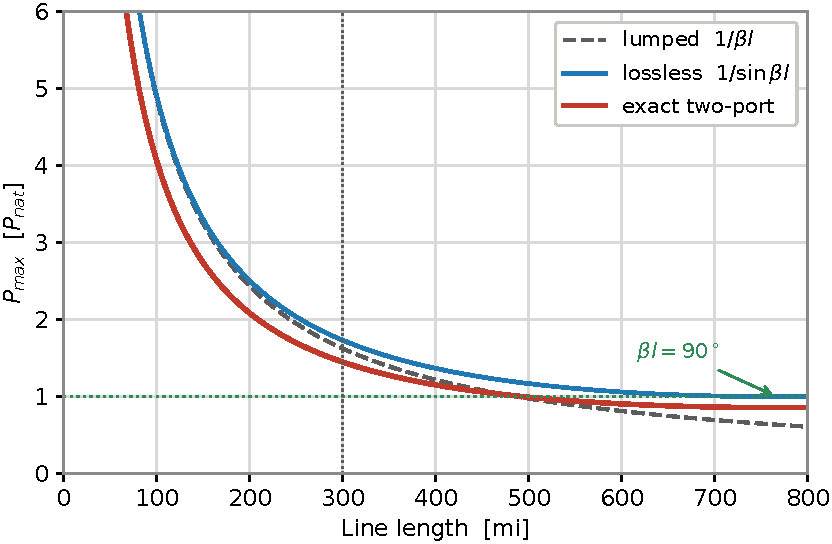
\includegraphics[width=0.74\linewidth]{ac-transmission/fig/as_electrical_length.pdf}
  \caption{Maximum transfer against length: lumped, lossless distributed and
           exact two-port}
  \label{fig:as-electrical-length}
\end{figure}

At the 300\,mi design length $\beta \cdot l = 35.2^\circ$, the lumped
reactance is $162.4\,\Omega$ against $X' = 153.4\,\Omega$, and
$1/\sin\left(\beta \cdot l\right) = 1.73$ against 1.45 for the exact
two-port; losses and charging account for the remaining gap.

\FloatBarrier

\subsubsection{Operating margin below the maximum}
\label{sec:as-contingency}

Two effects cut the usable transfer well below $P_{max}$, and they compound.

The first is the post-contingency network. Two parallel 300\,mi circuits
have $P_{max} = 2726$\,MW intact; losing one doubles the reactance of the
path and leaves 1363\,MW on the survivor. Planning practice requires a
margin of 30 to 35\,\% on the \emph{post-contingency} network,
\begin{equation}
  \frac{P_{max} - P}{P_{max}} \ge 0.30
  \label{eq:as-margin}
\end{equation}
which on this pair allows 954\,MW, or $1.02 \cdot P_{nat}$ for the two
circuits together. A transfer of 1200\,MW looks comfortable intact, at
$\delta = 22.9^\circ$, and sits only 12\,\% below the post-contingency
maximum --- not acceptable. For comparison, the thermal rating of the pair
is 6755\,MW, seven times the binding constraint.
Figure~\ref{fig:as-contingency} shows both power-angle curves.

\begin{figure}[!ht]
  \centering
  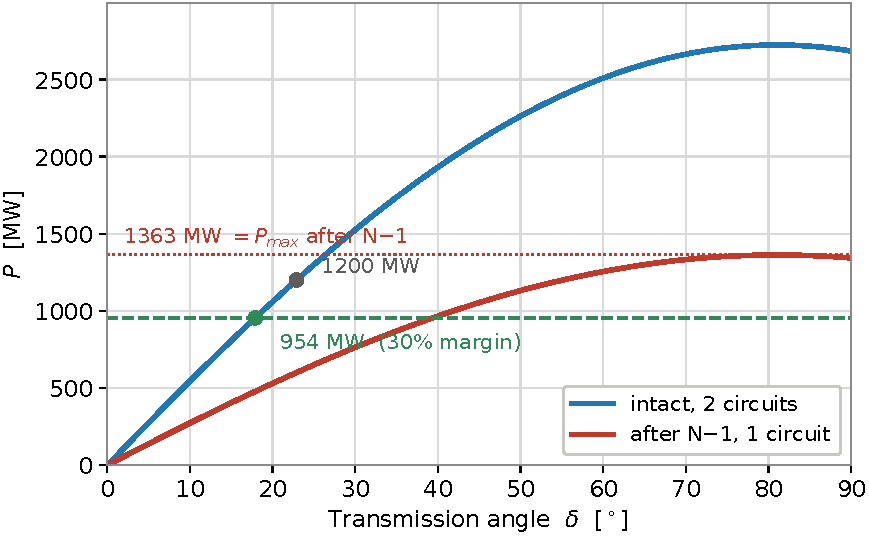
\includegraphics[width=0.74\linewidth]{ac-transmission/fig/as_contingency.pdf}
  \caption{Power-angle curves of two parallel 300\,mi circuits, intact and
           after the loss of one}
  \label{fig:as-contingency}
\end{figure}

\subsubsection{Transient stability}
\label{sec:as-equal-area}

The second effect is the fault case. During a fault the electrical output
collapses while the mechanical input continues; the rotor must give that
energy back before the maximum angle is reached. The equal-area criterion
states the condition as
\begin{equation}
  A_{acc} = \int_{\delta_0}^{\delta_{cc}}
            \left(P_m - P_{flt}\right) \mathrm{d}\delta
  \;=\;
  A_{dec} = \int_{\delta_{cc}}^{\delta_{max}}
            \left(P_{pst} - P_m\right) \mathrm{d}\delta
  \label{eq:as-equal-area}
\end{equation}
with $\delta_{cc}$ the clearing angle. For a machine at $P_m = 0.6$\,p.u.\
with maxima of 1.0 pre-fault, 0.3 during the fault and 0.7 after it,
$\delta_0 = 36.9^\circ$, $\delta_{cc} = 45.5^\circ$ and $\delta_{max} =
121.0^\circ$, Figure~\ref{fig:as-equal-area}.

\begin{figure}[!ht]
  \centering
  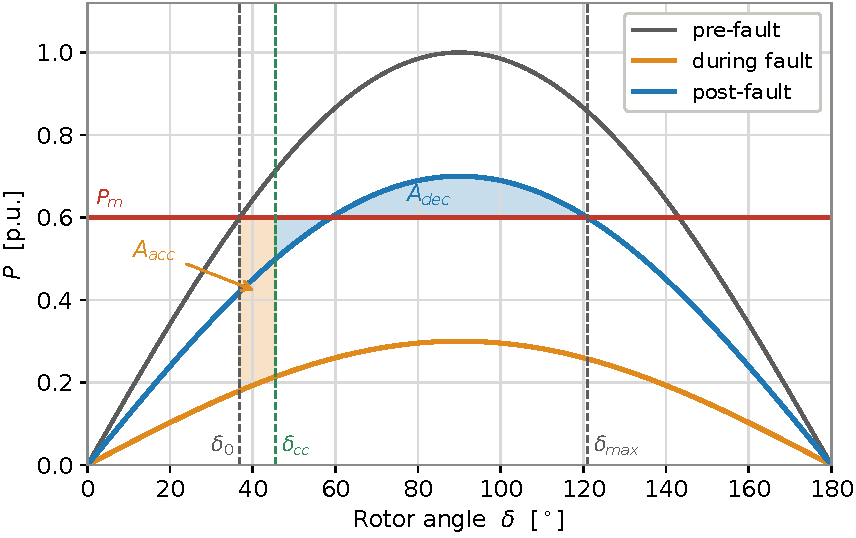
\includegraphics[width=0.72\linewidth]{ac-transmission/fig/as_equal_area.pdf}
  \caption{Equal-area criterion, generic machine per unit}
  \label{fig:as-equal-area}
\end{figure}

A higher pre-fault angle shrinks the decelerating area from both ends at
once, so the critical clearing time falls steeply with loading. This is why
two-cycle breakers and independent-pole tripping buy transfer capability,
and why the transient limit usually binds before the steady-state one.

\FloatBarrier

\subsubsection{Damping}
\label{sec:as-damping}

In a multi-machine system the classical limit generalises to an eigenvalue
criterion. The modes that constrain long transfers are the inter-area modes
at 0.2 to 0.8\,Hz; local plant modes at 0.8 to 2\,Hz and torsional modes at
10 to 45\,Hz. The practical limit is where the damping ratio of a critical
mode falls below about 3 to 5\,\%, which can occur at angles below
$40^\circ$ and therefore below the two-machine maximum.

High-gain automatic voltage regulators, which permit a large angle,
contribute \emph{negative} damping torque at heavy loading. The power system
stabiliser restores it. On a long corridor the available transfer is often
released by tuning the stabiliser rather than by raising $P_{max}$.

\subsubsection{Absence of a transmission angle on a DC link}
\label{sec:as-dc}

A DC link has no transmission angle, no synchronising torque and no
equal-area criterion. The converter control sets power as a commanded
quantity, and length enters only through the conductor resistance, so the
$1/\sin\left(\beta \cdot l\right)$ decay of~\eqref{eq:as-electrical-length}
has no counterpart. An embedded DC link can be modulated to damp the
inter-area modes of the surrounding AC system instead of loading them.

The constraint moves to the terminals: short-circuit ratio and commutation
robustness for line-commutated converters, control interaction for
voltage-sourced ones.

\FloatBarrier
